\chapter{Pattern Matching}\label{ch:pattern-matching}

Unter Pattern Matching versteht man im Allgemeinen den Abgleich von konkreten Strukturen mit Suchvorlagen.
Im Kontext dieser Arbeit soll speziell in Objektstrukturen nach bestimmten Mustern gesucht werden.
Dabei können Muster sowohl die Attribute von Objekten als auch Kanten zwischen diesen betreffen.
In diesem Kapitel werden drei Verfahren erläutert, welche die Definition von Mustern und deren Suche auf Objektenstrukturen erlauben.
Dafür wird zunächst die FulibTables\cite{fulibTables}-Bibliothek betrachtet, welche die Mustererkennung mit Java auf zwei verschiedene Weisen ermöglicht.
Darauf aufbauend wird eine Erweiterung der Scenario-Sprache vorgestellt, die Syntax zum Pattern Matching einführt.

\section{FulibTables}\label{sec:fulib-tables}

FulibTables ist eine Java-Bibliothek, mit der Objektstrukturen als Tabellen behandelt werden können.
Diese Tabellen dienen als Grundlage für einen Pattern Matcher, den die Bibliothek ebenfalls anbietet.
Im folgenden Abschnitt werden zunächst die Tabellen und deren Operationen anhand eines einfachen Beispiels vorgestellt.
Daraufhin werden die Möglichkeiten zum Pattern Matching mit FulibTables betrachtet.

\subsection{Tabellen}\label{subsec:tables}

Um Tabellen nutzen zu können, wird zunächst ein Datenmodell benötigt.
Dazu soll beispielhaft ein Modell von einem fiktiven Spiel für mehrere Spieler verwendet werden.
Jeder Spieler hat ein oder mehrere Häuser, die eine Zahl von Einheiten haben.
Ziel des Spiels ist es, in mindestens einem Haus eine bestimmte Anzahl von Einheiten zu erreichen.
Das entsprechende Klassendiagramm ist in Abbildung~\ref{fig:game-class-diagram} zu sehen.

\begin{figure}
    \centering
    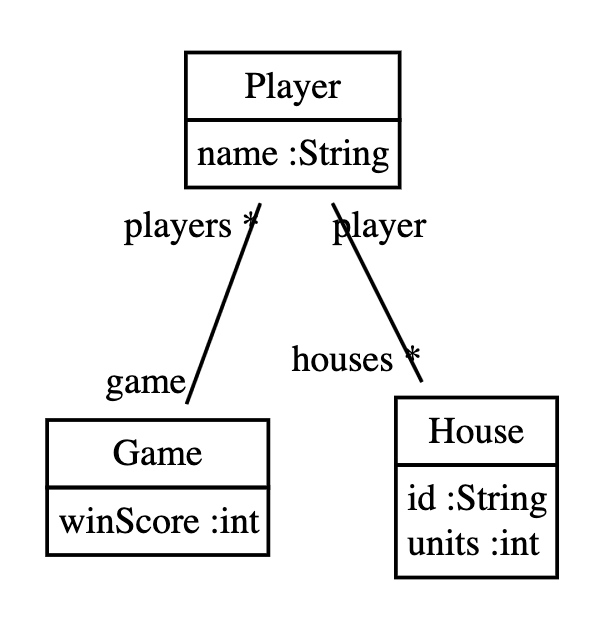
\includegraphics[width=0.4\textwidth]{chapter/pattern-matching/img/game-class-diagram.png}
    \caption{Beispiel-Klassendiagramm zur Verwendung von FulibTables}
    \label{fig:game-class-diagram}
\end{figure}

Es werden nun einige Beispielobjekte zu diesem Modell erstellt, die den Endzustand des Spiels beschreiben.
Das zugehörige Objektdiagramm ist in Abbildung~\ref{fig:game-object-diagram} zu sehen.

\begin{jcodeblock*}{breaklines}
    Game game = new Game().setWinScore(50);
    Player alice = new Player().setName("Alice").setGame(game);
    Player bob = new Player().setName("Bob").setGame(game);
    Player charlie = new Player().setName("Charlie").setGame(game);
    House a1 = new House().setId("a1").setUnits(30).setPlayer(alice);
    House a2 = new House().setId("a2").setUnits(20).setPlayer(alice);
    House b1 = new House().setId("b1").setUnits(40).setPlayer(bob);
    House c1 = new House().setId("c1").setUnits(60).setPlayer(charlie);
\end{jcodeblock*}

\begin{figure}
    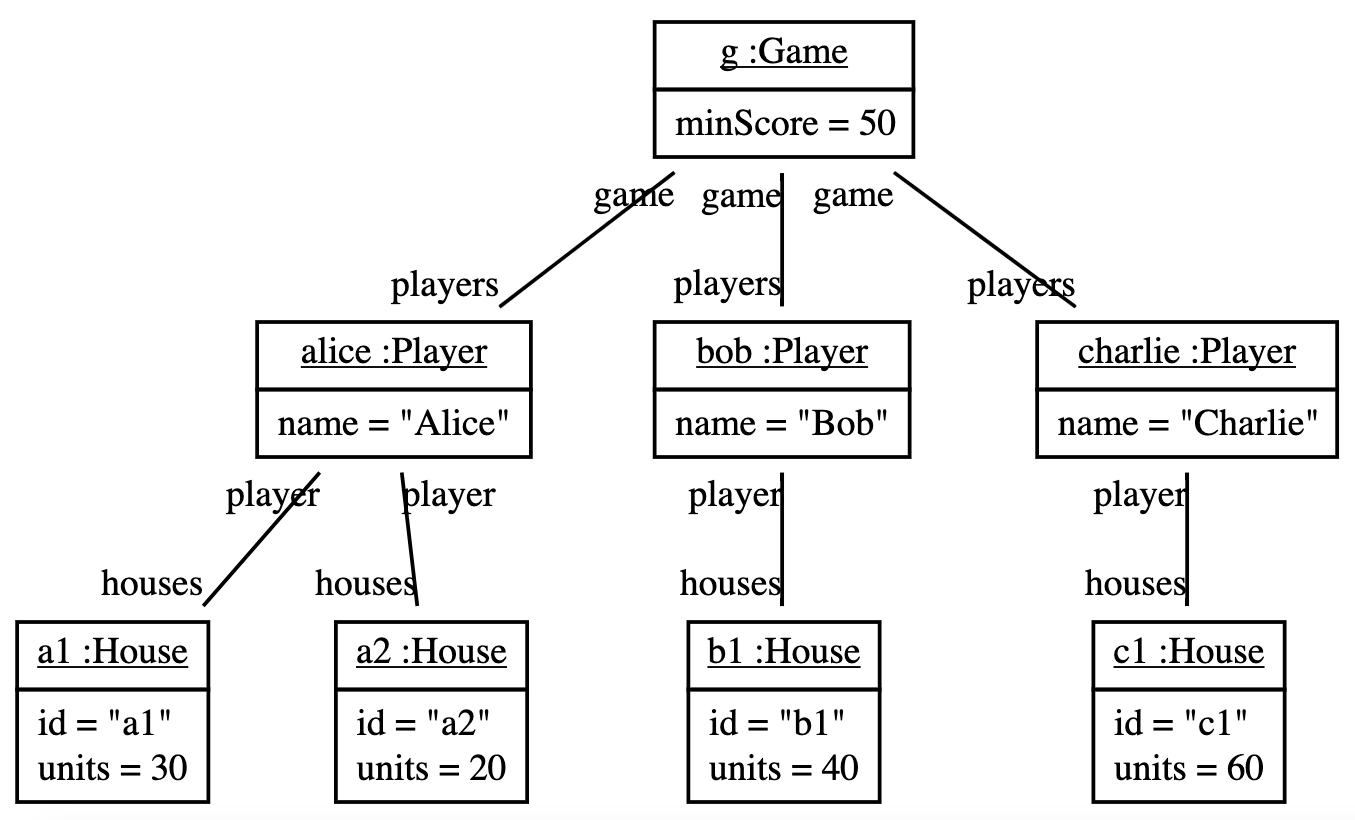
\includegraphics[width=\textwidth]{chapter/pattern-matching/img/game-object-diagram.png}
    \caption{Beispiel-Objektdiagramm zur Verarbeitung mit FulibTables}
    \label{fig:game-object-diagram}
\end{figure}

Nun kann eine Tabelle angelegt werden.
In FulibTables besteht jede Tabelle aus mindestens einer Spalte und null oder mehr Zeilen\footnote{Die Spaltennamen zählen dabei nicht als Zeile.}.
Tabellen können \emph{erweitert} oder \emph{eingeschränkt} werden, wobei Spalten entstehen oder entfernt werden\footnote{Die Einschränkung ist im Folgenden nicht näher erläutert, da sie für die hier verwendeten Beispiele keine Anwendung findet.}.
Beim Erweitern entstehen neue Tabellen-Instanzen, die sich die Daten der ursprünglichen Tabelle teilen.
Jede Tabellen-Instanz hat eine Spalte, auf die sie \emph{zeigt}.
Operationen auf der Tabelle beziehen sich in der Regel auf diese Spalte, wirken sich aber durch das geteilte Datenmodell auf alle verwandten Instanzen aus.
Das Objektdiagramm in Abbildung~\ref{fig:tables-object-diagram} zeigt, wie das Datenmodell von Tabellen aussehen kann und wie sich verschiedene Tabellen-Instanzen die Daten teilen.

\begin{figure}
    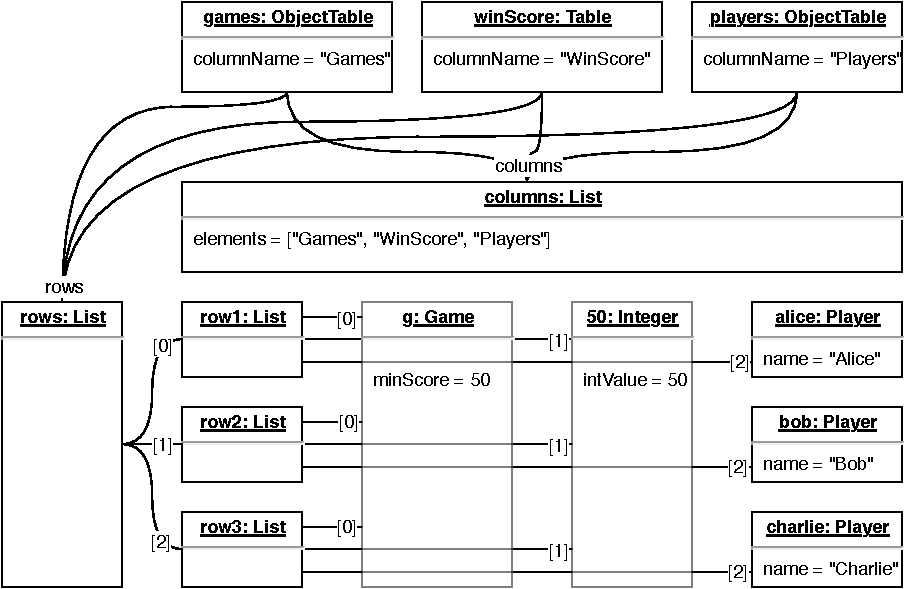
\includegraphics[width=\textwidth]{chapter/pattern-matching/img/tables-object-diagram.pdf}
    \caption{Objektdiagramm mehrerer Tabellen-Instanzen mit geteilten Daten}
    \label{fig:tables-object-diagram}
\end{figure}

Zunächst wird nur eine Tabelle mit einer Spalte und einer Zeile benötigt.
Dafür müssen der Name der ersten Spalte sowie eine Liste von Objekten, welche die Zeilen dieser Spalte bilden, angegeben werden.

\begin{jcodeblock}
    ObjectTable<Game> games = new ObjectTable<>("Game", game);
\end{jcodeblock}

Die Tabelle lässt sich wie folgt darstellen\footnote{FulibTables ermöglicht das Rendern von Tabellen als Markdown- und \ac{html}-Tabellen, die visuell den hier gezeigten Beispielen entsprechen.}:

\begin{tabular}{|c|}
    \hline
    \textbf{Game} \\
    \hline
    g \\
    \hline
\end{tabular}

Auf dieser Tabelle lässt sich nun eine Erweiterung durchführen, die mit der Methode \code{expand} erreicht wird.
Diese erwartet zuerst einen Namen für die neue Spalte, die der alten Tabelle hinzugefügt wird und auf welche die neue Tabellen-Instanz zeigen soll.
Weiterhin wird eine Funktion in Form eines Lambda-Ausdrucks übergeben.
Diese wird für jede Zeile der Tabelle aufgerufen.
Die Ergebnisse bilden dann die Zeilen der neuen Spalte.
Dies wird anhand des Beispiels deutlich:

\begin{jcodeblock*}{breaklines,escapeinside=||}
    Table<Integer> winScores = games.expand("Win Score", Game::getWinScore|\footnotemark|);
\end{jcodeblock*}
\footnotetext{Bei diesem Ausdruck handelt es sich um eine Methodenreferenz, die äquivalent zu dem Lambda-Ausdruck \jcode{game -> game.getWinScore()} ist.}

Die neue Tabelle lässt sich wie folgt darstellen:

\begin{tabular}{|c|c|}
    \hline
    \textbf{Game} & \textbf{Win Score} \\
    \hline
    g & 50 \\
    \hline
\end{tabular}

Die \code{expand}-Methode ist geeignet für Attribute und Zu-1-Assoziationen.
Für Zu-N-Assoziationen kommt die \code{expandAll}-Methode zum Einsatz.
Diese erwartet ebenfalls einen Spaltennamen und einen Lambda-Ausdruck, allerdings muss letzterer eine Liste von Werten zurückgeben.
Für jedes Element dieser Listen wird eine neue Zeile angelegt.

\begin{jcodeblock*}{breaklines}
    ObjectTable<Player> players = games.expandAll("Players", Game::getPlayers);
\end{jcodeblock*}

\begin{tabular}{|c|c|c|}
    \hline
    \textbf{Game} & \textbf{Win Score} & \textbf{Players} \\
    \hline
    g & 50 & Alice   \\
    g & 50 & Bob     \\
    g & 50 & Charlie \\
    \hline
\end{tabular}

Um das Verhalten zu verdeutlichen, wird eine weitere \code{expandAll}-Operation auf der entstandenen Tabelle durchgeführt.
Da Alice in diesem Beispiel zwei Häuser hat, wird ihre Zeile dupliziert.
Bei Bob und Charlie ist dies nicht der Fall.

\begin{jcodeblock*}{breaklines}
    ObjectTable<House> houses = players.expandAll("Houses", Player::getHouses);
\end{jcodeblock*}

\begin{tabular}{|c|c|c|c|}
    \hline
    \textbf{Game} & \textbf{Win Score} & \textbf{Players} & \textbf{Houses} \\
    \hline
    g & 50 & Alice   & a1 \\
    g & 50 & Alice   & a2 \\
    g & 50 & Bob     & b1 \\
    g & 50 & Charlie & c1 \\
    \hline
\end{tabular}

Wie im weiteren Verlauf dieses Kapitels gezeigt wird, ist der Name des zu erweiternden Attributs nicht immer bekannt.
Dafür wurde als Teil dieser Arbeit eine alternative \code{expandAll}-Operation entwickelt, bei der kein Lambda-Ausdruck übergeben wird und somit auch kein Name angegeben werden muss.
Stattdessen werden die existierenden Attribute und Assoziationen der Objekte zur Laufzeit ermittelt.
Dabei wird aus jedem Attributwert und jedem Assoziationsziel jedes Objekts der Spalte \code{Houses} eine neue Zeile.
Zu-N-Assoziationen und mehrwertige Attribute (Listen) werden dabei abgeflacht.

\begin{jcodeblock}
    Table<?> houseAttributes = houses.expandAll("House Attributes");
\end{jcodeblock}

\begin{tabular}{|c|c|c|c|c|}
    \hline
    \textbf{Game} & \textbf{Win Score} & \textbf{Players} & \textbf{Houses} & \textbf{House Attributes} \\
    \hline
    g & 50 & Alice   & a1 & a1      \\
    g & 50 & Alice   & a1 & Alice   \\
    g & 50 & Alice   & a1 & 30      \\
    g & 50 & Alice   & a2 & a2      \\
    g & 50 & Alice   & a2 & Alice   \\
    g & 50 & Alice   & a2 & 20      \\
    g & 50 & Bob     & b1 & b1      \\
    g & 50 & Bob     & b1 & Bob     \\
    g & 50 & Bob     & b1 & 40      \\
    g & 50 & Charlie & c1 & c1      \\
    g & 50 & Charlie & c1 & Charlie \\
    g & 50 & Charlie & c1 & 60      \\
    \hline
\end{tabular}

Die Zeilen einer Spalte können nun nach bestimmten Eigenschaften durchsucht werden.
Diese Operation nennt sich \code{filter} und verwendet ebenfalls einen Lambda-Ausdruck, der angibt, welche Zeilen entfernt und welche behalten werden sollen.
In diesem Beispiel wird unter allen Attributen der Häuser nach ganzen Zahlen gesucht.
Durch Auflisten aller Attribute und anschließendem Filtern kann eine Spalte für die Anzahl der Einheiten erstellt werden, ohne dass der Name des Attributs angegeben werden muss.

\begin{jcodeblock}
    houseAttributes.filter(it -> it instanceof Integer);
\end{jcodeblock}

\begin{tabular}{|c|c|c|c|c|}
    \hline
    \textbf{Game} & \textbf{Win Score} & \textbf{Players} & \textbf{Houses} & \textbf{House Attributes} \\
    \hline
    g & 50 & Alice   & a1 & 30      \\
    g & 50 & Alice   & a2 & 20      \\
    g & 50 & Bob     & b1 & 40      \\
    g & 50 & Charlie & c1 & 60      \\
    \hline
\end{tabular}

Alternativ kann auch eine Filterung über alle Spalten durchgeführt werden, wofür die \code{filterRows}-Operation eingesetzt wird.
Dieser wird ein Lambda-Ausdruck übergeben, der für jede Zeile die Werte aller Spalten erhält.
Die Werte befinden sich in einer \code{Map}, die einen Spaltennamen zu dem Wert in der aktuellen Zeile zuordnet.
Ist das Ergebnis des Lambda-Ausdrucks \jcode{true}, wird wie beim einfachen Filter die Zeile behalten, andernfalls wird sie entfernt.
In diesem Beispiel sorgt die Filter-Operation dafür, dass nur die Zeile mit dem Spieler Charlie übrig bleibt:

\begin{jcodeblock}
    houseAttributes.filterRows((Map<String, Object> row) -> {
        int winScore = (int) row.get("Win Score");
        int units = (int) row.get("House Attributes");
        return units >= winScore;
    });
\end{jcodeblock}

\begin{tabular}{|c|c|c|c|c|}
    \hline
    \textbf{Game} & \textbf{Win Score} & \textbf{Players} & \textbf{Houses} & \textbf{House Attributes} \\
    \hline
    g & 50 & Charlie & c1 & 60 \\
    \hline
\end{tabular}

Die Suche nach einem Gewinner ist nun abgeschlossen.
Aus der Tabelle lässt sich ein Ergebnis erzeugen, indem die Tabellenspalte \code{Players} in eine Liste konvertiert wird.

\begin{jcodeblock}
    System.out.println("the winner is: " + players.toList());
    // Output: the winner is: [Charlie]
\end{jcodeblock}

\subsection{Patterns}\label{subsec:patterns}

Patterns sind ein Mechanismus von FulibTables, der ähnlich wie Tabellen die Suche nach Objekten mit bestimmten Eigenschaften in einer Objektstruktur erlaubt.
Die Bibliothek gibt dafür eine einfache \ac{api} zum Konstruieren von Patterns vor.
Intern werden sie mit Tabellen realisiert, die Verwendung von Patterns ist jedoch übersichtlicher und leichter verständlich.
Des Weiteren werden Tabellen imperativ mit einer Folge von Anweisungen bearbeitet, während sich Patterns als Objekte modellieren und damit deklarativ gebrauchen lassen.

Ein Pattern besteht aus einer Menge von \emph{Pattern-Objekten} und \emph{Constraints} auf diesen.
Pattern-Objekte dienen als Platzhalter für Objekte und Werte, nach denen gesucht wird, während Constraints deren Beziehungen und Einschränkungen modellieren.

Es soll nun die zuvor mit Tabellen realisierte Suche nach einem Gewinner mit Patterns umgesetzt werden.
Das Datenmodell und die angelegten Objekte werden hier wiederverwendet.
Zunächst werden einige Pattern-Objekte benötigt, um die verschiedenen Arten von Objekten und Werten abzubilden.
Diese lassen sich mit einem \code{PatternBuilder} anlegen.

\begin{jcodeblock*}{breaklines}
    PatternBuilder builder = FulibTables.patternBuilder();

    PatternObject gamePO = builder.buildPatternObject("Game");
    PatternObject winScorePO = builder.buildPatternObject("WinScore");
    PatternObject playerPO = builder.buildPatternObject("Player");
    PatternObject housePO = builder.buildPatternObject("House");
    PatternObject unitsPO = builder.buildPatternObject("Units");
\end{jcodeblock*}

Pattern-Objekte werden nicht nur für Objekte im Datenmodell (\code{gamePO}, \code{playerPO}, \code{housePO}) benötigt, sondern auch für deren Attribute (\code{winScorePO} und \code{unitsPO}).
Intern entspricht jedes Pattern-Objekt einer Spalte der Tabelle, die am Ende des Match-Vorgangs alle Ergebnisse enthält.

Nun müssen die Pattern-Objekte verbunden werden.
Dies geschieht unter Angabe der Attribut- bzw.\ Assoziationsnamen mit der \code{buildPatternLink}-Methode.

\begin{jcodeblock}
    // Attribute:
    builder.buildPatternLink(gamePO, "winScore", winScorePO);
    // Assoziationen:
    builder.buildPatternLink(gamePO, "game", "players", playerPO);
    builder.buildPatternLink(playerPO, "player", "houses", housePO);
    // Beliebige Verknüpfung:
    builder.buildPatternLink(housePO, "*", unitsPO);
\end{jcodeblock}

Zu beachten ist in der letzten Zeile der Name ``\code{*}''.
Dieser dient als Platzhalter für einen unbekannten Attributnamen.
Er bewirkt, dass dem Pattern-Objekt \code{housePO} nur Objekte zugewiesen werden können, bei denen mindestens ein Attributwert auch \code{unitsPO} zugewiesen werden kann.
Die Unterstützung für den  ``\code{*}''-Platzhalter wurde als Teil dieser Arbeit entwickelt und baut auf der zuvor gezeigten \code{expandAll}-Operation auf.
Wie im vorherigen Beispiel sind nicht alle Attribute von Häusern interessant, weshalb auch hier auf ganze Zahlen eingeschränkt werden soll.
Dafür kommt ein \emph{Attribut-Constraint} zum Einsatz, das wie folgt angelegt wird:

\begin{jcodeblock*}{breaklines}
    builder.buildAttributeConstraint(unitsPO, it -> it instanceof Integer);
\end{jcodeblock*}

Maßgeblich für die Suche nach dem Gewinner ist die Bedingung, dass die Anzahl der Einheiten größer als das vom Spiel vorgegebene Minimum ist.
Analog zu \code{filterRows} bei Tabellen kommt dafür bei Patterns ein \emph{Match-Constraint} zum Einsatz, das wie folgt deklariert wird:

\begin{jcodeblock}
    builder.buildMatchConstraint(row -> {
        int winScore = (int) row.get("WinScore");
        int units = (int) row.get("Units");
        return units >= winScore;
    }, winScorePO, unitsPO);
\end{jcodeblock}

Der Lambda-Ausdruck entspricht hier jenem, der mit \code{filterRows} gebraucht wurde.
Zu beachten ist die darauffolgende Angabe der verwendeten Pattern-Objekte.
Im Allgemeinen können Match-Constraints erst dann verarbeitet werden, wenn alle von ihnen verwendeten Pattern-Objekte gefunden wurden.
Wären diese nicht explizit angegeben, müsste davon ausgegangen werden, dass das Match-Constraint \emph{alle} Pattern-Objekte verwendet.
Dann müssten zunächst alle Pattern-Objekte zugewiesen werden, bevor das Match-Constraint verarbeitet werden kann.
Dabei könnten jedoch große Zwischenergebnisse entstehen, was zu erheblich längeren Ausführungszeiten führen kann.

Nun sind alle Pattern-Objekte und Constraints angelegt.
Mit \code{builder.getPattern()} lässt sich ein Objekt erhalten, dass all diese kapselt.
Damit kann nun der Match-Vorgang durchgeführt werden.
Dafür wird zunächst ein \code{PatternMatcher} benötigt, der mit \code{new PatternMatcher(builder.getPattern())} erstellt werden kann.
Alternativ kann er auch direkt mit dem \code{builder} angelegt werden, wie das untenstehende Beispiel zeigt.
Dem Matcher werden dann ein oder mehr \emph{Root-Objekte} und \emph{Root-Pattern-Objekte} zugewiesen.
Diese entsprechen den Objekten und Pattern-Objekten, bei denen die Suche begonnen wird.
Ferner werden daraus die initialen Zeilen und Spalten der Tabelle, die intern als Datenstruktur dient.

\begin{jcodeblock}
    PatternMatcher matcher = builder.matcher();
    matcher.withRootPatternObjects(gamePO);
    matcher.withRootObjects(game);
    matcher.match();
\end{jcodeblock}

Die Methode \code{match()} führt nach Einrichten des Matchers den eigentlichen Match-Vorgang durch.
Dabei werden ausgehend von der internen Tabelle nacheinander die Attribut-, Link- und Match-Constraints angewendet.
Dies erfolgt durch Ausführung der \code{filter}-, \code{expand} / \code{expandAll} und \code{filterRows}-Operationen auf der Tabelle.
Die Reihenfolge wird automatisch so gewählt, dass zu jedem Zeitpunkt möglichst wenige Tabellenzeilen entstehen, um den Aufwand gering zu halten.
Dazu werden Attribut-\ und Match-Constraints, welche die Zeilenanzahl nur verringern können, den Link-Constraints, die neue Spalten und Zeilen erzeugen, vorgezogen.
Link-Constraints werden immer erst dann verarbeitet, wenn weder Attribut-\ noch Match-Constraints anwendbar sind.
Durch die automatische Optimierung haben Patterns den Vorteil, dass der Nutzer sich anders als mit Tabellen nicht die Reihenfolge der Operationen überlegen muss, sondern sich auf die Suchkriterien konzentrieren kann.

Nach dem Match-Vorgang lassen sich die Ergebnisse anhand der Pattern-Objekte extrahieren:

\begin{jcodeblock}
    Player winner = matcher.findOne(playerPO);
    System.out.println("the winner is: " + winner);
\end{jcodeblock}

Die \code{findOne}-Methode stellt sicher, dass es auch wirklich genau ein Objekt gibt, das \code{playerPO} zugewiesen ist.
Gäbe es keinen Spieler, der das Minimum an Einheiten erreicht hat, würde sie eine \code{NoMatchException} werfen.
Andererseits würde die Existenz mehrerer solcher Spieler eine \code{AmbiguousMatchException} verursachen.
Möchte man dies erlauben, kann stattdessen \code{findAll} verwendet werden.
Dies gibt eine Menge aller gematchten Objekte zurück, die auch leer sein kann.

\begin{jcodeblock}
    Set<Player> winners = matcher.findAll(playerPO);
\end{jcodeblock}

\section{Pattern Matching in der Scenario-Sprache}\label{sec:scenario-pattern-matching}

Die Scenario-Sprache bietet syntaktische Unterstützung für Pattern Matching mit FulibTables in Form des \emph{Match-Satzes}.
Er erlaubt es, in einer kompakten und ausdrucksstarken Weise Patterns zu bauen und auf Objektstrukturen anzuwenden.
Ergebnisse des Satzes sind die gefundenen Objekte, die im weiteren Verlauf des Scenarios verwendet werden können.
Seine umfangreiche Syntax ist Thema dieses Abschnitts.

Ein Match-Satz ist an dem Schlüsselwort \code{match} bzw.\ \code{matches} erkennbar, dem ein Subjekt voransteht.
Es folgt eine Liste von Pattern-Objekten, die an den Schlüsselwörten \code{some} und \code{all} zu erkennen sind.
Das folgende Beispiel zeigt den einfachsten möglichen Match-Satz, der nach genau einem Objekt sucht und es an den Namen \code{g} bindet.

\begin{mdcodeblock}
    There is a Game.

    We match some object g.
\end{mdcodeblock}

Dieser einfache Satz generiert vergleichsweise langen Java-Code, wie nachfolgend zu sehen ist.
Es handelt sich dabei um genau jenen Code, der zur Einrichtung von Patterns und eines Matchers sowie zur Extraktion von Ergebnissen aus diesem benötigt wird.

\begin{jcodeblock*}{breaklines}
    Object g;
    {
        // Pattern
        PatternBuilder builder = FulibTables.patternBuilder();
        PatternObject gPO = builder.buildPatternObject("g");
        // Matcher
        PatternMatcher matcher = builder.matcher();
        matcher.withRootPatternObjects(gPO);
        matcher.withRootObjects(new ReflectorMap("org.example").discoverObjects(game)); // (1)
        matcher.match();
        // Results
        g = matcher.findOne(gPO);
    }
\end{jcodeblock*}

Eine Besonderheit ist der Aufruf von \code{withRootObjects} bei \code{(1)}.
Der Aufruf von \code{discoverObjects} bewirkt in diesem Beispiel, dass alle von \code{game} ausgehenden Objekte, deren Typ zum Package \code{org.example} gehört, als Root-Objekte behandelt werden.
Dies umfasst \code{game} selber sowie alle über direkte und transitive Assoziationen verknüpften Objekte, demnach die gesamte Objektstruktur.
Der Scenario-Compiler sammelt alle sich im Scope befindenden Variablen und übergibt sie an \code{discoverObjects}.
Die Methode stellt sicher, dass auch Objekte gefunden werden, die nicht direkt zugänglich sind.
Wichtig ist jedoch, dass nicht direkt nach Objekten gesucht werden kann, die nicht zum Package des Scenarios gehören.
Dies schließt insbesondere einfache Werte wie Zahlen oder Strings als Root-Objekte aus.

\subsection{Typ-Constraints}

Statt \code{object} lässt sich im Match-Satz auch ein Typ angeben, auf den das Pattern-Objekt beschränkt sein soll.

\begin{mdcodeblock}
    We match some Game g.
\end{mdcodeblock}

Dies wirkt sich auf das Pattern-Objekt im Java-Code aus.

\begin{jcodeblock}
    PatternObject gPO = builder.buildPatternObject("g", Game.class);
    // äquivalent zu:
    // PatternObject gPO = builder.buildPatternObject("g");
    // builder.buildAttributeConstraint(gPO, g -> g instanceof Game);
\end{jcodeblock}

Typ-Constraints können nützlich sein, wenn statt nach \emph{einem} Objekt nach \emph{allen} Objekten eines Typs gesucht wird.
Dafür kann statt \code{some} das Schlüsselwort \code{all} verwendet werden:

\begin{mdcodeblock}
    There is a Player with name Alice.
    There is a Player with name Bob.

    We match all players ps.
\end{mdcodeblock}

Dadurch wird \code{ps} zu einer Liste, die mittels \code{findAll} vom Matcher erhalten wird:

\begin{jcodeblock}
    List<Player> ps;
    {
        // ...
        ps = matcher.findAll(psPO);
    }
\end{jcodeblock}

Die Liste lässt sich wie gewohnt im Scenario weiterverwenden:

\begin{mdcodeblock}
    We take some player from ps and ...
\end{mdcodeblock}

\subsection{Attribut-Constraints mit Gleichheit}

Auf Pattern-Objekte in Match-Sätzen folgt eine Liste von Constraints.
Eine einfache Art davon ist ein Attributwert-Constraint.
Wie das folgende Beispiel zeigt, verwendet dieser eine ähnliche Syntax wie Attribute in There-Sätzen.

\begin{mdcodeblock}
    There is a Game with min-score 50.

    We match some object g with min-score 50.
\end{mdcodeblock}

Durch Hinzunahme des Constraints entsteht im Java-Code ein weiteres Pattern-Objekt, das mit dem Pattern-Objekt von \code{g} über ein Link-Constraint verbunden ist und durch ein Gleichheits-Constraint eingeschränkt wird.

\begin{jcodeblock*}{breaklines,escapeinside=||}
    Object g;
    {
        PatternBuilder builder = FulibTables.patternBuilder();
        PatternObject gPO = builder.buildPatternObject("g");
        PatternObject gMinScorePO = builder.buildPatternObject("gMinScore");
        builder.buildPatternLink(gPO, "minScore", gMinScore);
        builder.buildEqualityConstraint(gMinScorePO, 60)|\footnotemark|;
        // Matcher, Results...
    }
\end{jcodeblock*}
\footnotetext{Dieser Aufruf ist äquivalent zu \jcode{builder.buildAttributeConstraint(gMinScorePO, gMinScore -> gMinScore == 60);}.}

\subsection{Attribut-Constraints mit Vergleichsoperatoren}

Attributwert-Constraint müssen nicht nach exakten Werten prüfen.
Sie können stattdessen auch mit bestimmten Bedingungen wie etwa Zahlenvergleichen oder regulären Ausdrücken eingeschränkt werden.
Die Syntax ändert sich dabei leicht durch Verwendung des Schlüsselworts \code{whose}.

\begin{mdcodeblock}
    There is a Player with name Alice.

    We match some object g whose min-score is greater than 0.
    We match some object p1 whose name matches '[Aa]lice'.
\end{mdcodeblock}

Im Java-Code wird aus dem Gleichheits-Constraint ein allgemeiner Attribut-Constraint mit einem Lambda-Ausdruck.
Durch die Verwendung als Operand wird der Typ der Attribut-Pattern-Objekte eingeschränkt, um die Voraussetzungen des Operators zu erfüllen.

\begin{jcodeblock*}{breaklines}
    PatternObject gMinScorePO = builder.buildPatternObject("gMinScore", Number.class);
    builder.buildAttributeConstraint(gMinScorePO, (Number n) -> n.doubleValue() > 0);

    PatternObject p1NamePO = builder.buildPatternObject("p1Name", String.class);
    builder.buildAttributeConstraint(p1NamePO, (String s) -> s.matches("[Aa]lice"));
\end{jcodeblock*}

\subsection{Attribut-Constraints mit unbekannten Attribut-Namen}

Die vorherigen Beispiele setzen voraus, dass der Name des Attributs bekannt ist.
Match-Sätze erlauben jedoch auch, eine Bedingung an ein beliebiges Attribut zu stellen, dessen Name nicht bekannt ist.
Als Platzhalter dient dafür \code{some attribute};
das Schlüsselwort \code{whose} wird zu \code{where}.

\begin{mdcodeblock}
    There is a Player with username Alice.

    We match some object p1 where some attribute matches '[Aa]lice'.
\end{mdcodeblock}

Nun ist die Benennung des Attributes nicht mehr entscheidend, solange der Wert passend ist.
Statt \code{username} könnte das Attribut auch \code{label} oder \code{nickname} heißen.
Im Java-Code verändert sich primär das Link-Constraint zwischen den beiden Pattern-Objekten, indem der im vorherigen Abschnitt erklärte Platzhalter \code{*} verwendet wird.

\begin{jcodeblock*}{breaklines}
    PatternObject p1Attr1PO = builder.buildPatternObject("p1Attr1", String.class);
    builder.buildPatternLink(p1PO, "*", p1AttrPO);
    // AttributeConstraint... (s.o.)
\end{jcodeblock*}

\subsection{Mehrere Root-Objekte und Fehlerfälle}

Link-Constraints kommen auch zum Einsatz, wenn nach Assoziationen zwischen Objekten gesucht wird.
Dafür werden zunächst zwei Pattern-Objekte benötigt.
In einem Match-Satz müssen diese lediglich durch \code{and} oder Komma getrennt werden:

\begin{mdcodeblock}
    We match some object g and some object p1.
\end{mdcodeblock}

% Unordered List syntax
Eine alternative Schreibweise verwendet jedoch eine Auflisting der Pattern-Objekte mit der Markdown-eigenen Syntax für ungeordnete Listen.
Diese ist aufgrund der Leserlichkeit der einzeiligen Schreibweise vorzuziehen.

\begin{mdcodeblock}
    We match:
    - some object g
    - some object p1.
\end{mdcodeblock}

% Mehrere Root-POs
Beide Schreibweisen bewirken, dass sowohl nach \code{g} als auch nach \code{p1} unter allen Root-Objekten gesucht wird.

\begin{jcodeblock}
    matcher.withRootPatternObjects(gPO, p1PO);
\end{jcodeblock}

% Ungleichheits-Bedingung
Ferner impliziert die Existenz mehrerer Pattern-Objekte im gleichen Match-Satz, dass diese ungleich sein müssen.
Genau diese Ungleichheits-Bedingung bewirkt, dass die reine Deklaration mehrerer Pattern-Objekte \emph{nicht} gleichbedeutend mit der Verwendung mehrerer Match-Sätze ist\footnote{Ein Beispiel mit mehreren Match-Sätzen wäre: \code{We match some object g. We match some object p1.}.}.

\begin{jcodeblock}
    builder.buildDistinctConstraint(gPO, p1PO);
\end{jcodeblock}

% Exceptions
Konkret hat dies die Konsequenz, dass \code{g} und \code{p1} in keinem Fall das selbe Objekt matchen können.
Ohne weitere Einschränkung kann mit diesem Beispiel kein erfolgreiches Match erzielt werden, unabhängig davon welche Objekte davor erstellt werden.
Wird vor dem Match-Satz nur genau ein Objekt deklariert, kann dieses entweder \code{g} oder \code{p1} zugewiesen werden, aber nicht beiden Pattern-Objekten gleichzeitig.
Dies bewirkt ein Fehlschlagen des Match-Vorgangs mit einer \code{NoMatchException}.
Wenn mehrere Objekte wie beispielsweise \code{game} und \code{Alice} deklariert werden, sind sowohl \code{g=game, p1=Alice} als auch \code{g=Alice, p1=game} mögliche Zuweisungen des Patterns.
Diese Uneindeutigkeit bewirkt, dass der Match-Vorgang mit einer \code{AmbiguousMatchException} abbricht.
Durch Wiedereinführung des Attribut-Constraints des Spielernamens kann das Problem behoben werden.
Damit wird die eindeutige Zuweisung \code{g=game, p1=Alice} erzwungen.

\subsection{Link-Constraints}

% Some Link To
Es soll nun nach einer Verknüpfung zwischen den andernfalls unabhängigen Objekten gesucht werden.
Ist der Name der Assoziation unwichtig oder unbekannt, kommt das Constraint \code{with some link to} zum Einsatz:

\begin{mdcodeblock}
    We match:
    - some object g with some link to p1
    - some object p1 where some attribute matches '[Aa]lice'.
\end{mdcodeblock}

% Beliebige Reihenfolge
Hier ist besonders zu beachten, dass ein Pattern-Objekt vor dessen Deklaration referenziert werden kann.
Dies ist durch die deklarative Natur des generierten Java-Codes möglich, da zuerst alle Pattern-Objekte und dann deren Constraints erstellt werden.
Auch hier wird statt eines konkreten Verknüpfungsnamens der Platzhalter \code{*} eingesetzt.

\begin{jcodeblock}
    PatternObject gPO = builder.buildPatternObject("g");
    PatternObject p1PO = builder.buildPatternObject("p1");
    builder.buildPatternLink(gPO, "*", p1PO); // some link to
    // AttributeConstraint...
\end{jcodeblock}

\subsection{Benannte Link-Constraints mit Attribut-Constraints}

% Named Links with Attribute Constraints
Bei Link-Constraints kann auch der Name der Assoziation angegeben werden.
Dies ist möglich, indem man die Syntax für Attribute verwendet, aber statt eines Werts den Namen eines Pattern-Objekts angibt:

\begin{mdcodeblock}
    We match:
    - some object g with players p1
    - some object p1 where some attribute matches '[Aa]lice'.
\end{mdcodeblock}

Der Java-Code errinnert stark an jenen, der zuvor für das reguläre Attribut-Constraint generiert wurde:

\begin{jcodeblock}
    final PatternObject gPO = builder.buildPatternObject("g");
    final PatternObject p1PO = builder.buildPatternObject("p1");
    builder.buildPatternLink(gPO, "players", p1PO);
\end{jcodeblock}

% Attributes as POs
Der wesentliche Unterschied ist, dass zuvor das Attribut-Pattern-Objekt \code{gMinScore} nur der Einschränkung diente und nach dem Match-Vorgang verworfen wurde, \code{p1PO} jedoch auch an die Variable \code{p1} gebunden wird und somit später verfügbar ist.
Diese Eigenschaft lässt sich auch für Attribute nutzen, deren Wert später zugänglich gemacht werden soll.
So kann durch Hinzufügen eines explizit benannten Root-Pattern-Objekts der Wert von \code{minScore} ermittelt werden:

\begin{mdcodeblock}
    We match:
    - some object g with min-score ms
    - some integer ms
    We expect that ms is 50.
\end{mdcodeblock}

Statt \code{with min-score} kann auch \code{where some attribute is} eingesetzt werden, wenn der Name des Attributs nicht bekannt ist.
Ferner wäre auch \code{with some link to} einsetzbar und in diesem Beispiel semantisch äquivalent zu \code{where some attribute is}.
Davon ist jedoch abzuraten, da es sich bei \code{ws} um einen Wert und kein Objekt im Sinne der Modellierung handelt, weshalb die Bezeichnung ``Link'' irreführend wäre.

\subsection{Match-Constraints}

Auch Match-Constraints werden von der Scenario-Sprache in Match-Sätzen unterstützt.
Dafür kommt erneut das Schlüsselwort \code{where} zum Einsatz.
Darauf folgt ein Bedingungsausdruck, der beliebig viele Pattern-Objekte aus dem gleichen Match-Satz enthalten kann.

\begin{mdcodeblock*}{breaklines}
    We match:
    - some game g
    - some player p1
    where min-score of g is 0 or score of p1 is greater than min-score of g.
\end{mdcodeblock*}

Im Java-Code ist ersichtlich, dass automatisch die Abhängigkeit des Match-Constraints von den Pattern-Objekten \code{g} und \code{p1} erkannt wurde.
Im Bedingungsausdruck wurden deren Namen durch Hilfsvariablen ersetzt, da die eigentlichen Variablen erst nach Abschluss des Match-Vorgangs verfügbar sind.

\begin{jcodeblock*}{breaklines}
    builder.buildMatchConstraint(row -> {
        Game _g = (Game) row.get("g");
        Player _p1 = (Player) row.get("p1");
        return _g.getMinScore() == 0 || _p1.getScore() > _g.getMinScore();
    }, gPO, p1PO);
\end{jcodeblock*}

Mit einem Match-Constraint lässt sich auch das Beispiel aus dem vorherigen Unterabschnitt ausstatten, um das Attribut \code{minScore} einzuschränken.
Dies war zuvor syntaktisch nicht mehr möglich.

\begin{mdcodeblock}
    We match:
    - some object g with min-score ms
    - some integer ms where ms is greater than 0
\end{mdcodeblock}
